\begin{surferPage}{Another Cusp ($A_2^{++}$ Singularity)}
This singularity is similar to the previous cusp--singularity.
    Its equation is exactly the same except that a sign has changed:
    \vspace*{-0.4em}
    \begin{center}
      $x^3+y^2+z^2=0.$
    \end{center}
    \vspace*{-0.4em} 
    This change of sign causes the surface to be rotation--symmetric, 
    as is its deformation with equation 
    $(1-a)x^3-ax^2+y^2+z^2=0$, $a>0$ into a singularity of type $A_1^{+-}$: 
    \begin{center}
      \vspace*{-0.7em}
      \begin{tabular}{@{}c@{\quad}c@{\quad}c@{}}
        \begin{tabular}{@{}c@{}}
          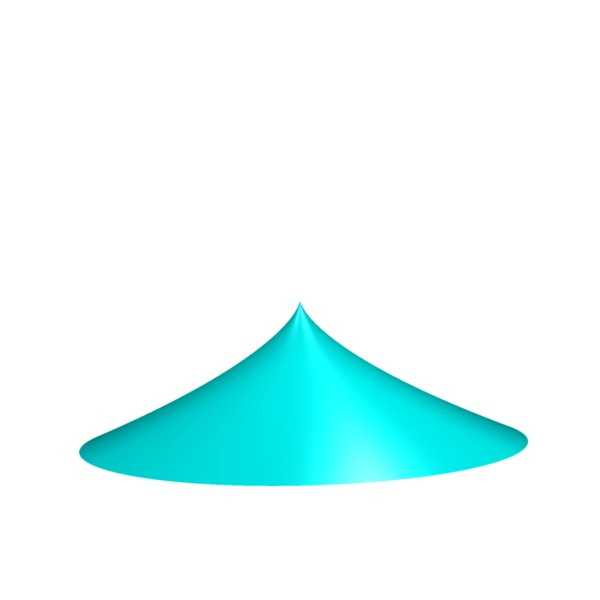
\includegraphics[width=1.2cm]{../../common/images/A2pp_0}
        \end{tabular}
        &
        \begin{tabular}{@{}c@{}}
          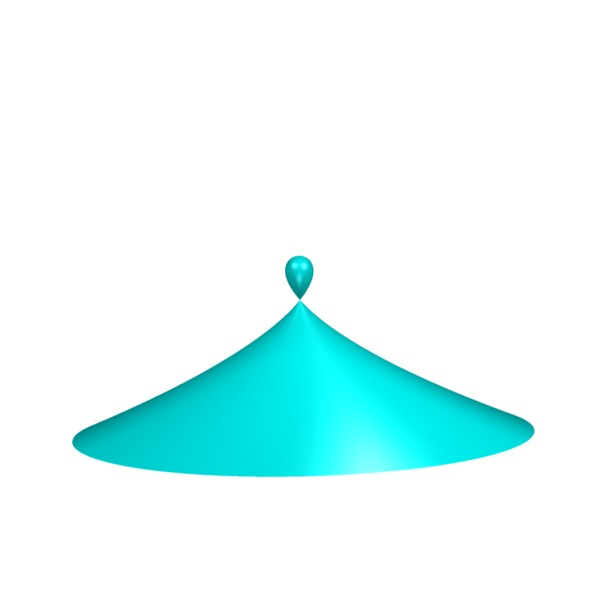
\includegraphics[width=1.2cm]{../../common/images/A2pp_1}
        \end{tabular}
        &
        \begin{tabular}{@{}c@{}}
          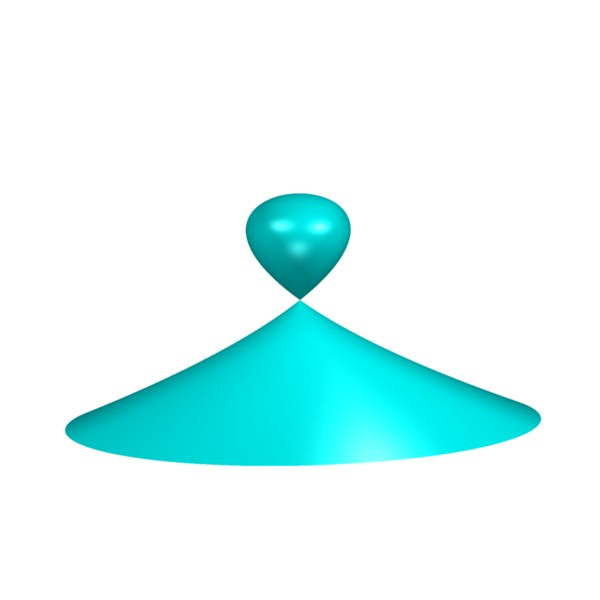
\includegraphics[width=1.2cm]{../../common/images/A2pp_2}
        \end{tabular}
      \end{tabular}
    \end{center}
    \vspace*{-0.4em}
    The rotation--symmetry in the $yz$--plane can be seen easily:
    Writing the equation in the form $y^2+z^2=-(x^3)$, we see that for each
    fixed value $x<0$ we obtain a circle, because the equation $y^2+z^2=r^2$
    describes a circle with radius $r$ by the Pythagorean Theorem.  
    
    Cutting the deformed cusp with a plane, we get a plane cusp and a loop:
    \begin{center}
      \vspace*{-0.7em}
      \begin{tabular}{@{}c@{\quad}c@{\quad}c@{}}
        \begin{tabular}{@{}c@{}}
          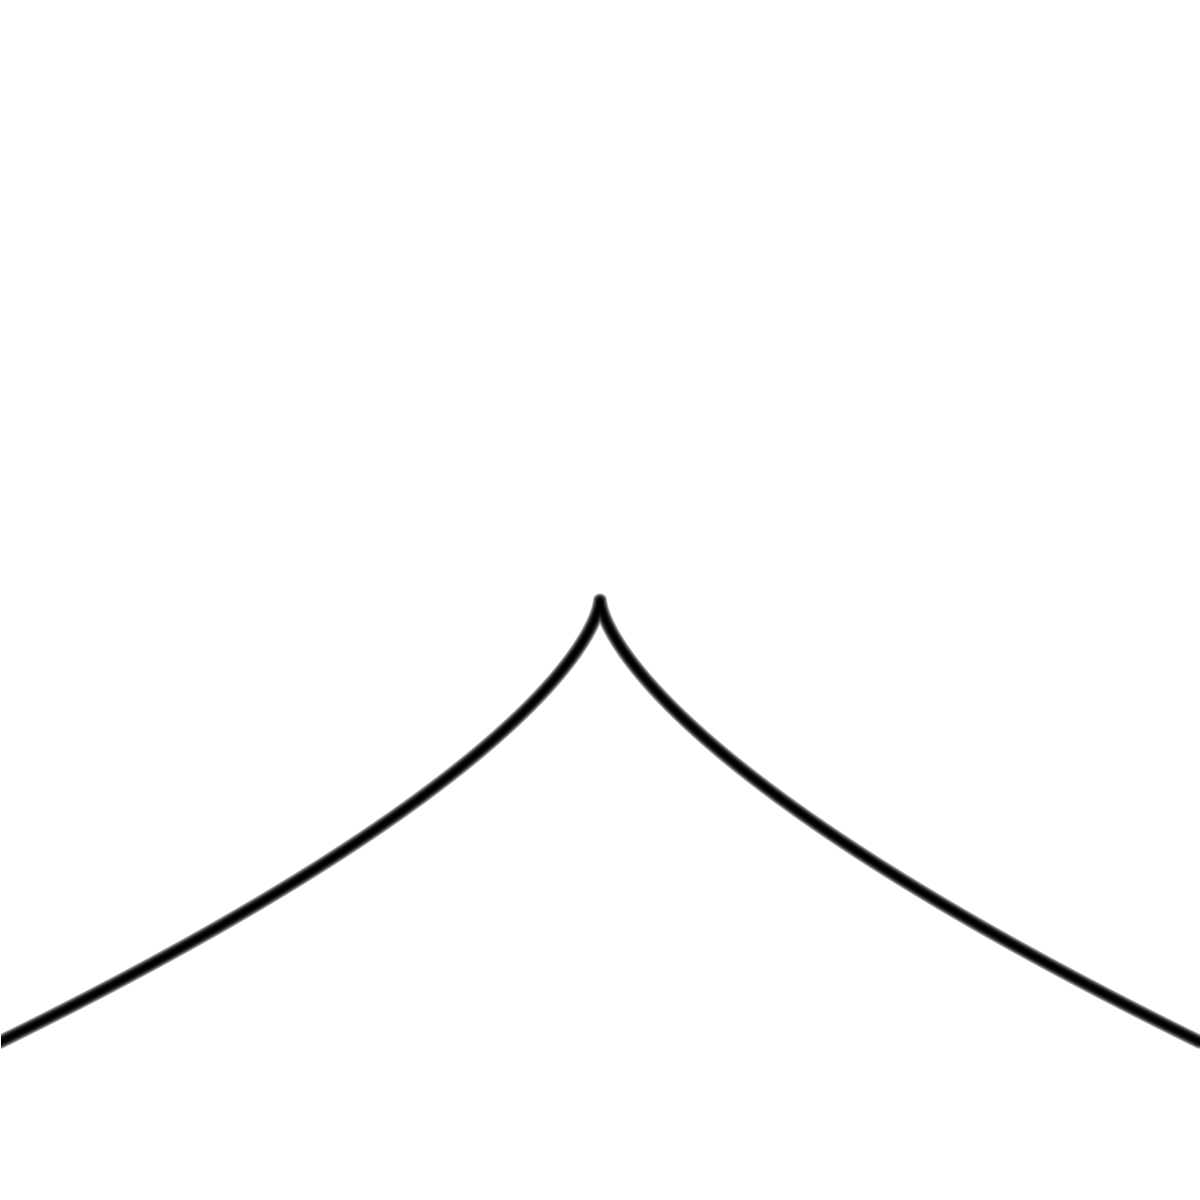
\includegraphics[width=1.2cm]{../../common/images/cuspe_def_cut_1}
        \end{tabular}
        &
        \begin{tabular}{@{}c@{}}
          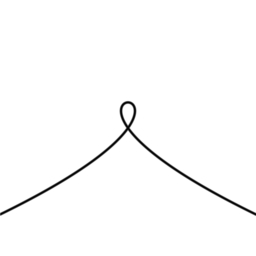
\includegraphics[width=1.2cm]{../../common/images/cuspe_def_cut_2}
        \end{tabular}
        &
        \begin{tabular}{@{}c@{}}
          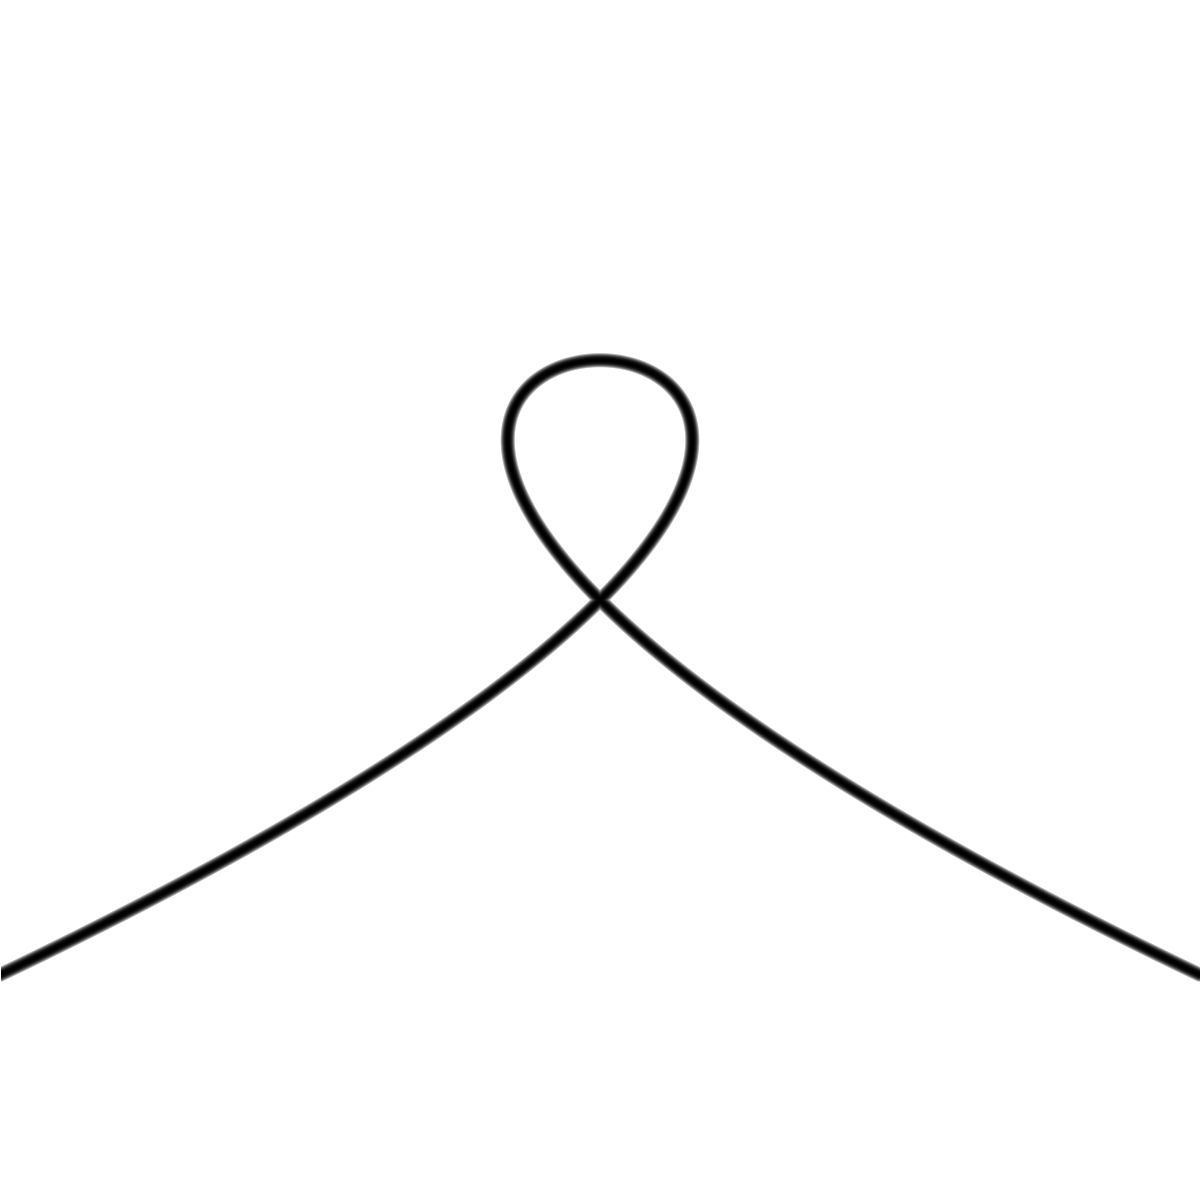
\includegraphics[width=1.2cm]{../../common/images/cuspe_def_cut_3}
        \end{tabular}
      \end{tabular}
    \end{center}
 
\end{surferPage}
